\chapter{Day 3: Linear Independence, Span, Basis, and Decomposition}

\section{Schedule}
\begin{itemize}
\item 0900-0930: Debrief and Dancing Animal Demos
\item 0930-1000: Synthesis 
\item 1000-1030: Mini-Lecture: Linear Independence, Span, Basis, Decomposition
\item 1030-1045: Coffee
\item 1045-1210: Technical Details: Linear Independence, Span, Basis, Decomposition
\item 1210-1220: Preview
\end{itemize}

\section{Debrief and Dancing Animal Demos}

\bi
\item Please discuss your overnight work with your table-mates, create a set of key concepts, and a set of ideas that you are still confused by.
\item Be prepared to demo your dancing animal!
\ei

\section{Synthesis}

\begin{prob}
You should do all of these.
\be
\item Assume the matrix $\mathbf{D}$ represents a geometrical object. What is the correct matrix expression if we want to rotate it first ($\R$), then scale it ($\S$), and finally translate ($\T$) it?

\begin{tabular}{ll}
A. $\mathbf{D} \R \S \T$ \\
B. $\T \S \R \mathbf{D}$ \\
C. $\R \S \T \mathbf{D}$ \\
D. $\mathbf{D} \T \S \R$
\end{tabular}

\item What would be the correct expression in order to undo the transformation in the previous problem?

\item $\A$ and $\mathbf{B}$ are square, invertible matrices of the same size. Which of the following are \textbf{always} true (no matter the entries in $\A$ and $B$? 

\begin{tabular}{l}
A. $(\A \mathbf{B})^T = \mathbf{B}^T \A^T$ \\
B. $(\A \mathbf{B})^{-1} = \mathbf{B}^{-1} \A^{-1}$ \\
C. $(\A^T)^{-1} = (\A^{-1})^T$ \\
D. $\det(\A \mathbf{B}) = \det(\A) \det(\mathbf{B})$ \\
E. $\A + \mathbf{B} = \mathbf{B} + \A$ \\
F. $\A \mathbf{B} = \mathbf{B} \A$ \\
G. $\det(\A \mathbf{B}) = \det(\A) + \det(\mathbf{B})$ \\
H. $(\A \mathbf{B})^T = \A^T \mathbf{B}^T$ \\
I. $(\A \mathbf{B})^{-1} = \A^{-1} \mathbf{B}^{-1}$
\end{tabular}
\ee
\end{prob}

% \begin{prob}
% It would be really good to complete these questions.
% \be
% \item Consider the following linear system of algebraic equations 
% \begin{eqnarray*}
% x + y &=& 1 \\
% 2x + hy &=& k 
% \end{eqnarray*}
% where $h$ and $k$ are real numbers that can be varied (parameters).
% \be
% \item Using any technique you know of, go ahead and "solve" for $x$ and $y$ by hand.
% \item Write this linear system of algebraic equations in matrix-vector form $\A \x = \b$.
% \item Find the determinant of $\A$. Under what conditions is det$(\A)=0$? det$(\A)\ne0$?
% \item Use the inverse of $\A$ to find the solution $\x$ in the case where det$(\A) \ne 0$.
% \item Match the following terms

% \begin{tabular}{ll}
% i. No Solution & A. $h \ne 2$, any $k$ \\
% ii. Infinite Solutions & B. $h=2$ and $k=2$ \\
% iii. Unique Solution & C. $h=2$ and $k \ne 2$
% \end{tabular}

% and explain the situations corresponding to "No Solution" and "Infinite Solution".
% \ee
% \ee
% \end{prob}

\section{Linear Independence, Span, and Decomposition}

\begin{prob}
Consider two column vectors
\begin{align}
\mathbf{a}_1 = \threebyone{1}{1}{0}, \;\mathbf{a}_2 = \threebyone{1}{2}{0}
\end{align}
Both these vectors lie on the $xy$-plane since their $z$ components are zero. Define a new vector $\mathbf{a}_3 = c_1\mathbf{a}_1 + c_2\mathbf{a}_2$, where $c_1$ and $c_2$ are arbitrary variables. Therefore $\mathbf{a}_3$ is a linear combination of $\mathbf{a}_1$ and $\mathbf{a}_2$.
\begin{enumerate}
\item Does $\mathbf{a}_3$ also lie on the $xy$-plane?
\item Next, define a $3\times 3$ matrix $\mathbf{A}$ whose columns are $\mathbf{a}_1$, $\mathbf{a}_2$ and $\mathbf{a}_3$. Show that the product of $\mathbf{A}$ and any $3\times 1$ vector always lies on the $xy$-plane.
\end{enumerate}
\end{prob}
\begin{sol}
	\begin{enumerate}
		\item Yes, a linear combination of two vectors which lie in the $xy$-plane will also lie in the $xy$-plane.
		\item Let $\mathbf{A}$ be the matrix
		$$\mathbf{A} = \begin{bmatrix} 1 & 1 & c_1+c_2 \\ 1 & 2 & c_1+2c_2 \\ 0 & 0 & 0 \end{bmatrix}$$
		and let $\mathbf{v}$ be an arbitrary $3 \times 1$ vector
		$$\mathbf{v} = \begin{bmatrix} x \\ y \\ z \end{bmatrix}.$$
		Then the product
		$$\mathbf{Av} = \begin{bmatrix} x + y + (c_1+c_2)z \\ x + 2y + (c_1+2c_2)z \\ 0 \end{bmatrix}$$
		lies in the $xy$-plane
		\end{enumerate}
\end{sol}

\begin{prob}
Next, we will do a similar problem, but in MATLAB. Consider the following matrix:
\begin{align}
\mathbf{B} = \threebythree{1}{1}{3}{1}{2}{4}{1}{1}{3}
\end{align}
The third column of this matrix equals the second column plus twice the first column.  Hence these three vectors lie on some plane (not the $xy$-plane as in the previous part).
\begin{enumerate}
\item Open up MATLAB and using the \texttt{quiver3} command together with \texttt{hold on}, please plot the vectors corresponding to the three columns of $\mathbf{B}$, e.g., to plot the first column, type \texttt{>> quiver3(0,0,0, 1,1,1);} in MATLAB.
\item  Using the "rotate 3D" function on the MATLAB figure window, rotate the figure around so that it appears as if all three arrows overlap. This should indicate that the vectors lie on a plane.
\item Using \texttt{det} compute the determinant of matrix $\mathbf{B}$. Does this make sense?
\end{enumerate}
\end{prob}
\begin{sol}
	\begin{enumerate}
		\item Type the following into MATLAB:\\
		\texttt{>> quiver3(0,0,0,1,1,1)}\\
		\texttt{>> hold on}\\
		\texttt{>> quiver3(0,0,0,1,2,1)}\\
		\texttt{>> quiver3(0,0,0,3,4,3)}
		\item 
		\item The determinant of $\mathbf{B}$ is zero. Recall that a matrix is not invertible if and only if the determinant is zero. This matrix is not invertible since it collapses all vectors to a plane.
	\end{enumerate}
\end{sol}

The fundamental property here is that the columns of the $\A$ and $\mathbf{B}$ matrices are not \emph{linearly independent}. We shall next define the idea of linearly independent vectors more formally.

\begin{itemize}
\item A finite set $S = \{\x_1,\x_2,\ldots,\x_m\}$ of vectors in $\R^n$ is said to be \textit{linearly dependent} if there exist scalars $c_1, c_2, \ldots, c_m$ which are  not all zero,  such that
\[ c_1 \x_1 + c_2 \x_2 + \ldots + c_m \x_m = \mathbf{0}. \] Note that $\R^n$ here refers to the set of all $n$-dimensional vectors that are made up of real numbers. (For example, $\mathbf{R}^1$ is the real line and $\mathbf{R}^2$ is the plane.) For any value of $n$, $\R^n$ is an example of a \textit{vector space} - we will meet different examples of vector spaces in the future. We can also express this equation using a matrix $\mathbf{A}$, whose columns are $\x_1, \x_2, \cdots \x_m$.
\begin{align}
\begin{bmatrix}\x_1 & \x_2 & \hdots & \x_m \end{bmatrix} \threebyone{c_1}{\vdots}{c_m} = \mathbf{0}\,.
\end{align}
If a non-zero solution exists to $\A \mathbf{c} = \mathbf{0}$ then the set of vectors $\x_1,\x_2,\ldots,\x_m$ is linearly dependent. In the case of a square matrix ($n = m$), the vectors $\x_1, \x_2, \cdots \x_m$ are linearly dependent if and only if the $\det(\A) = 0$. Otherwise, the only way to satisfy the equation above is if $c_1 = c_2 = \cdots = c_m = 0$. Figure \ref{figDependentVectors} illustrates two examples of three vectors that are in 3D space, but are linearly dependent, since in each case, all three vectors are on a plane.

\begin{center}
  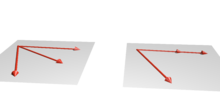
\includegraphics[width=0.5\textwidth]{FacesDay3/figs/Vec-dep.png}
  \captionof{figure}{Linearly dependent vectors in $\R^3$. (from Wikimedia Commons).}
  \label{figDependentVectors}
\end{center}

\item The set of vectors $\x_1,\x_2,\ldots,\x_m$ is \textit{linearly independent} if it is not linearly dependent. In other words, the set of vectors $\x_1,\x_2,\ldots,\x_m$ is linearly independent if
\begin{align}
c_1 \x_1 + c_2 \x_2 + \ldots + c_m \x_m = \mathbf{0}\,
\end{align}
only when $c_1 = c_2  = \cdots  = c_m = 0$. In other words, if the only solution to $\A \mathbf{c} = \mathbf{0}$ is $\mathbf{c} = \mathbf{0}$,
 the set of vectors  made up of the columns of $\A$ is linearly independent. For a square matrix this means the set is linearly independent if and only if $\det(\A) \ne 0$.

\begin{center}
  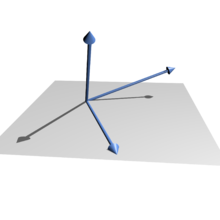
\includegraphics[width=0.5\textwidth]{FacesDay3/figs/Vec-indep.png}
  \captionof{figure}{Linearly independent vectors in $\R^3$. (from Wikimedia Commons).}
  \label{figIndependentVectors}
\end{center}

\item The \textit{span} of $S$ is the set of all linear combinations of its vectors. In other words, the span of the set $S$ is the set of all possible vectors of the form
\[ c_1 \x_1 + c_2 \x_2 + \ldots + c_m \x_m  \]
The \textit{span} is usually denoted by $span(\x_1,\x_2,\ldots,\x_m)$.

\item  A finite set $S = \{\x_1,\x_2,\ldots,\x_m\}$ of vectors is said to form a basis of a vector space $V$, if the vectors in $S$ are linearly independent, and every point in $V$ can be expressed as a linear combination of the vectors in the set $S$. Hence, if a set of vectors $S$ is linearly independent those vectors form a \textit{basis} of the set which is the span of those vectors.
\end{itemize}

Let's solidify our understanding of linear dependence, bases and span  by working on a few problems by hand.

\begin{prob}
\begin{enumerate}
    \item Determine which of the following sets of vectors are linearly independent.
\begin{enumerate}
\item \threebyone{1}{0}{0},  \threebyone{0}{1}{0},  \threebyone{0}{0}{2}
\item \threebyone{1}{3}{0},  \threebyone{1}{1}{0},  \threebyone{0}{1}{0}
\item \threebyone{1}{2}{3},  \threebyone{1}{1}{0},  \threebyone{3}{4}{3}
\item $\mathbf{p}$, $\mathbf{q}$, $\mathbf{r}$ and $\mathbf{s}$, where the vectors are all 3-dimensional. 
\item \twobyone{1}{2}, \twobyone{3}{3}
\end{enumerate}
\item In words, describe the span of the vectors \twobyone{1}{1} and \twobyone{1}{-1}.
\item In words, describe the span of the vectors \threebyone{1}{1}{0}, \threebyone{2}{3}{0} and \threebyone{1}{-1}{0} which are all in 3-dimensional Euclidean space. 
\end{enumerate}
\end{prob}
\begin{sol}
\begin{enumerate}
	\item \begin{enumerate}
		\item They are linearly independent since they span $\mathbf{R}^3$.
		\item They are linearly dependent since the first vector is equal to the second vector plus two times the third vector.
		\item They are linearly dependent since the third vector is equal to the first vector plus two times the second vector.
		\item They are linearly dependent. You can have a maximum of $n$ linearly independent vectors in $\mathbf{R}^n$.
		\item They are linearly independent since they do not lie on the same line.
	\end{enumerate}
	\item The span of these two vectors is all over $\mathbf{R}^2$, i.e., a plane.
	\item The span of these three vectors is the $xy$-plane in $\mathbf{R}^3$.
\end{enumerate}
\end{sol}

\subsection{Orthogonality}

\begin{center}
  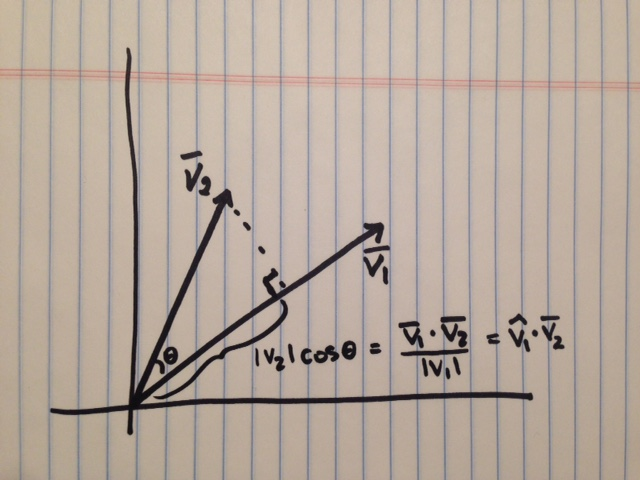
\includegraphics[width=0.5\textwidth]{FacesDay3/figs/Projection.jpg}
  \captionof{figure}{Projection}
\end{center}

By trigonometry, if we have two vectors ${\mathbf v}_1$ and ${\mathbf v}_2$ which have an angle of $\theta$ between them, the component of ${\mathbf v}_2$ which lies along the direction of ${\mathbf v}_1$ is $|\v_2| \cos{\theta}$.  Since the dot product of the two vectors can be expressed as $|\v_1||\v_2| \cos{\theta}$, this component (referred to as the projection) can be written as ${\mathbf v}_1 \cdot {\mathbf v}_2/|\v_1|$. If the projection is zero, the vectors are \textit{orthogonal}, and ${\mathbf v}_1 \cdot {\mathbf v}_2 = 0$. If the vectors are unit length, in addition to being normal, the vectors are said to be \emph{orthonormal}. Additionally, if a basis set is made up of orthonormal vectors, it is known as an orthonormal basis.

A square matrix with columns of unit vectors which are orthogonal to each other is known as an orthogonal matrix. An orthogonal marix $\mathbf{A}$ has the property that ${\mathbf{A}}^T = {\mathbf{A}}^{-1}$.

\begin{prob}
Which of the following pairs of vectors are orthogonal or orthonormal?
\begin{enumerate}
\item \threebyone{1}{2}{3}, \threebyone{-3}{2}{1}
\item \threebyone{1}{0}{-3}, \threebyone{3}{2}{1}
\item \twobyone{{\frac{2}{\sqrt{13}}}}{{\frac{-2}{\sqrt{13}}}}, \twobyone{{\frac{-3}{\sqrt{13}}}}{{\frac{3}{\sqrt{13}}}}
\end{enumerate}
\end{prob}
\begin{sol}
	\begin{enumerate}
		\item The dot product of these two vectors is non-zero, so they are not orthogonal.
		\item The dot product of these two vectors is zero, so they are orthogonal.
		\item The dot product of these two vectors is zero, so they are orthogonal. Furthermore, each vector is unit length, so they are orthonormal.
	\end{enumerate}
\end{sol}

\subsection{Decomposition}

Suppose we have a set (collection) of $m$ basis vectors $\{ {\mathbf v}_i \}$ which are normalized ($ |\v_i| = 1$), mutually orthogonal (${\mathbf v}_i ^T {\mathbf v}_j = 0$ unless $i=j$) and span our space (every point can be written as some linear combination of the vectors $\{ {\mathbf v}_i \}$).  How do we actually find the linear combination which is equal to a given vector in our space?

Let's say we have a vector ${\mathbf w}$ which we are interested in expressing as a linear combination of our set of orthonormal vectors $\{ {\mathbf v}_i \}$.  We can write this linear combination as
\begin{equation}
{\mathbf w} = \sum_{i=1}^m c_i {\mathbf v}_i
\end{equation}
and our problem is now to find the coefficients $c_i$ in this expression.

The obvious option is to pack the basis vectors $\v_i$ into the columns of a matrix $\A$, and find solutions of
\[ \A \mathbf{c} = \mathbf{w} \]
Since the columns of $\A$ are formed from basis vectors they are linearly independent and a non-zero solution exists and can be determined by the usual methods.

However, our basis vectors form an orthogonal set (collection) which permits a more direct calculation. Consider  a particular vector ${\mathbf v}_k$ in our basis set, and let's take the dot product between $\mathbf{v}_k$ and our vector $\mathbf{w}$:
\begin{equation}
{\mathbf v}_k^T {\mathbf w} = {\mathbf v}_k ^T\sum_{i=1}^m c_i {\mathbf v}_i
\end{equation}
Distributing the dot product into the summation we have:
\begin{equation}
{\mathbf v}_k^T {\mathbf w} = \sum_{i=1}^m c_i {\mathbf v}_k^T{\mathbf v}_i
\end{equation}
But from orthogonality we know that the dot product of any two different vectors in our orthonormal set is zero, so all terms in the sum where $k \neq i$ are zero. This leads to the following simplification
\begin{equation}
{\mathbf v}_k^T {\mathbf w} = c_k {\mathbf v}_k^T {\mathbf v}_k
\end{equation}
In addition, since our set of vectors is normalized, we know that ${\mathbf v}_k^T {\mathbf v}_k = 1$, leaving us with
\begin{equation}
{\mathbf v}_k^T {\mathbf w} = c_k
\end{equation}
This gives us a very nice, simple way of decomposing a vector into a linear combination of the vectors within our basis set.  The dot product of each basis vector with our target vector will result in the coefficient of that term in the linear decomposition.

\begin{prob}
\begin{enumerate}
\item There are many (in general, an infinite number) of bases for a given set $V$. Hence, we can describe elements in the set $V$ as linear combinations of vectors from different bases. Consider the following two basis sets which form bases for 2-dimensional space.
   \begin{itemize}
       \item
        $\mathbf{v}_1 = \twobyone{1}{0}, \ \mathbf{v}_2 = \twobyone{0}{1}$  and
    \item
        $\mathbf{u}_1 = \twobyone{\frac{1}{\sqrt{2}}}{\frac{1}{\sqrt{2}}}, \ \mathbf{u}_2 = \twobyone{-\frac{1}{\sqrt{2}}}{\frac{1}{\sqrt{2}}}$
    \end{itemize}

    Express the vector $\mathbf{w} = \twobyone{2}{3}$ as a linear combination of the first basis set (i.e., a sum of scaled versions of each vector in the basis set). Repeat for the second. Please make two different drawings of $\twobyone{2}{3}$, one expressed as a sum of scaled vectors in the first basis set and another for the vectors from the second basis set. Please label the lengths of each vector in the set.


\item Suppose that you wish to write the vector $\mathbf{w} =\threebyone{1}{2}{4}$ as a linear combination of the vectors
$$\mathbf{v}_1 =\threebyone{1}{1}{1}, \ \mathbf{v}_2=\threebyone{3}{1}{2} \text{ and } \mathbf{v}_3=\threebyone{1}{2}{2}.$$
 Please write a matrix equation to find the coefficients of the linear combination, and solve for the coefficients using MATLAB if possible.



\item Representing vectors using different bases is a very powerful technique that we will keep coming back to in this class (in both semesters). Vectors described in different bases can give us insight that may not be so obvious when viewed in the original basis.  Representing vectors in different bases can also be used for dimensionality reduction, which is an important technique that is used to speed up computations and compress data in a number of different fields. Here we will consider a problem of lossy data compression using a change of basis. Lossy compression refers to methods of representing data more efficiently, but with a loss of accuracy. Examples of lossy data compression include jpg images, and mp3 audio files.     If care is taken in lossy compression, the effects of the data loss can be kept at acceptable levels (this is of course subjective and dependent on the application). We will start with a toy example and then move to  more complicated ones in subsequent homework problems.
    Consider a set of four 2-dimensional data variables stored in the following vectors:



    \begin{align}
    \mathbf{d}_1 = \twobyone{2.2}{1.2} , \mathbf{d}_2 = \twobyone{1}{0.6}, \mathbf{d}_3 = \twobyone{1.5}{0.7}, \mathbf{d}_4 = \twobyone{1.7}{0.8}
    \end{align}


    \begin{enumerate}
    \item In MATLAB, plot the data using points (without lines connecting them) by typing \texttt{plot([2.2 1 1.5 1.7],[1.2 0.6 0.7 0.8], 'o');} You will find that these points lie close to the line through the origin with slope 1/2.

    \item  Define a unit vector that points in the direction $\twobyone{2}{1}$ and call it $\u_1$. Find another unit vector that is orthogonal to $\u_1$ and call it $\u_2$. These vectors form a basis in 2 dimensional space.

    \item Rather than storing the original data, we are now going to express the original data in terms of the new basis that we have defined. To do that, write $\mathbf{d}_1, \mathbf{d}_2, \mathbf{d}_3$ and $\mathbf{d}_4$, as a linear combination of $\u_1$ and $\u_2$. You can use MATLAB here to find the coefficients.

    \item In this toy example, we are going to "compress" our data by only keeping the coefficients corresponding to $\u_1$. i.e. we will discard the coefficient corresponding to $\u_2$. Suppose that we wish to recover approximations to $\mathbf{d}_1, \mathbf{d}_2, \mathbf{d}_3, \mathbf{d}_4$, from the four coefficients. These approximations, which you should denote by $\tilde{\mathbf{d}}_1, \cdots \tilde{\mathbf{d}}_4$, are all scaled versions of $\u_1$. In your axes from part a, please plot the points corresponding to $\tilde{\mathbf{d}}_1, \cdots \tilde{\mathbf{d}}_4$. Do you think they make good approximations?

    \item We can describe how well our compressed data represents our original data. One way to do this is to calculate the difference between our original and compressed data, and call this error vector $\mathbf{f_i}=\mathbf{d}_i - \tilde{\mathbf{d}}_i$. Now, compute the size of this error using $norm(\mathbf{f_i})$ for $i = 1, 2, 3, 4$. Then, summarize the error by finding the root-mean-square (RMS) error between your approximations and the true data points. The RMS function squares the errors, takes the mean, and then takes the square root. This quantity is a single number that can be used to measure how well or poorly your compressed data represents your original data. You may find MATLAB's \texttt{norm} and \texttt{rms} functions helpful here.
    \end{enumerate}
    This toy example illustrates that we can sometime be more efficient (albeit at the cost of some accuracy) in representing (or computing) data when it is expressed in certain bases.
\end{enumerate}
\end{prob}
\begin{sol}
	\begin{enumerate}
		\item It's clear that $2\mathbf{v}_1 + 3\mathbf{v}_2 = \mathbf{w}$. We visualize this as
		\begin{center}
    \begin{tikzpicture}[scale=.7]
    \draw [<->,gray!50!black] (0,0) --(0,4) node[left]{};
    \draw [->,gray!50!black] (0,0)--(4,0) node[right]{};

    \draw [->,red] (0,0)--(2,3) node[above] {$\mathbf{w}$};
    \draw [->,blue] (0,0)--(2,0) node[below] {$2\mathbf{v}_1$};
    \draw [->,blue] (2,0)--(2,3) node[left] {$3\mathbf{v}_2$};

    \end{tikzpicture}
    \end{center}
		
		
		To write $\mathbf{w}$ as a linear combination of the basis vectors $\mathbf{u}_1$ and $\mathbf{u}_2$ requires a bit more work. We can set up the matrix equation
		$$\begin{bmatrix} \frac{1}{\sqrt{2}} & \frac{-1}{\sqrt{2}} \\ \frac{1}{\sqrt{2}} & \frac{1}{\sqrt{2}} \end{bmatrix}\begin{bmatrix} c_1 \\ c_2 \end{bmatrix} = \begin{bmatrix} 2 \\ 3 \end{bmatrix}$$
		and solve to learn that $\frac{5}{\sqrt{2}}\mathbf{u}_1 + \frac{1}{\sqrt{2}}\mathbf{u}_2 = \mathbf{w}$. We can visualize this as
		
	\begin{center}
    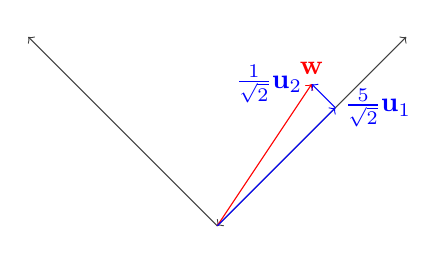
\begin{tikzpicture}[scale=.6]
    \draw [<->,gray!50!black] (0,0) --(4,4) node[left]{};
    \draw [->,gray!50!black] (0,0)--(-4,4) node[right]{};

    \draw [->,red] (0,0)--(2,3) node[above] {$\mathbf{w}$};
    \draw [->,blue] (0,0)--(2.5,2.5) node[right] {$\frac{5}{\sqrt{2}}\mathbf{u}_1$};
    \draw [->,blue] (2.5,2.5)--(2,3) node[left] {$\frac{1}{\sqrt{2}}\mathbf{u}_2$};

    \end{tikzpicture}
    \end{center}
    
    \item First, we create a matrix in MATLAB whose columns are the vectors $\mathbf{v}_1$, $\mathbf{v}_2$, and $\mathbf{v}_3$,\\
    \texttt{>> V=[1 3 1; 1 1 2; 1 2 2]}\\
    and the vector $\mathbf{w}$,\\
    \texttt{>> w=[1; 2; 4]}.\\
    Let $\mathbf{c}$ be the vector of coefficients. We have the equation $\mathbf{Vc}=\mathbf{w}$, so to solve for $\mathbf{c}$ we compute $\mathbf{c} = \mathbf{V}^{-1}\mathbf{w}$. In MATLAB, we use \texttt{>> inv(V)*w}. This tells us that $\mathbf{w} = -10\mathbf{v}_1 + 2\mathbf{v}_2 + 5\mathbf{v}_3$.
    
    \item \begin{enumerate}
        \item 
        \item We define \texttt{>> u1=[2; 1]} and \texttt{>> u2=[-1; 2]}. There are other choices for $\mathbf{u}_2$, but they are all constant multiples of this choice, e.g., \texttt{>> u2=[-2;4]}.
        \item Create a $2 \times 2$ matrix with $\mathbf{u}_1$ and $\mathbf{u}_2$ as the columns,\\
        \texttt{>> U=[2 -1; 1 2]}\\
        and a $2 \times 4$ matrix the vectors $\mathbf{d}_i$ as the columns\\
        \texttt{>> D=[2.2 1 1.5 1.7; 1.2 0.6 0.7 0.8]}.\\
        Then compute\\
        \texttt{>> inv(U)*D}\\
        to get the matrix of coefficients. This tells us that $$\mathbf{d}_1=1.12\mathbf{u}_1+0.04\mathbf{u}_2, \ \mathbf{d}_2=0.52\mathbf{u}_1+0.04\mathbf{u}_2,$$ $$\mathbf{d}_3=0.74\mathbf{u}_1-0.02\mathbf{u}_2, \text{ and } \mathbf{d}_1=0.84\mathbf{u}_1-0.02\mathbf{u}_2.$$
    \end{enumerate}
		
	\end{enumerate}
\end{sol}

\pagebreak
\shipoutAnswer